%!TeX root=../tese.tex
\chapter{Álgebras de flag}
\label{cap:flag-algebras}


\newcommand{\rfsigma}{\mathbb{R}\mathcal{F}^\sigma}
\newcommand{\asigma}{\mathcal{A}^\sigma}

\newcommand{\emptyflag}{\varnothing}
\newcommand{\isom}{\cong}

% Tikz setup from https://arxiv.org/abs/2103.14179


\newcommand{\vc}[1]{\ensuremath{\vcenter{\hbox{#1}}}}
\tikzset{vtx/.style={inner sep=1.7pt, outer sep=0pt, circle, fill}}
\tikzset{unlabeled_vertex/.style={inner sep=1.7pt, outer sep=0pt, circle, fill, draw=black}}
\tikzset{labeled_vertex/.style={inner sep=2.2pt, outer sep=0pt, rectangle, fill=yellow, draw=black}}
\tikzset{edge_color0/.style={color=black,line width=1.2pt}}
\tikzset{edge_color1/.style={color=red,  line width=1.2pt,opacity=0}}
\tikzset{edge_color2/.style={color=blue, line width=1.2pt,opacity=1}}

\newcommand{\flagone}{ % this is the unlabeled triangle
  \vc{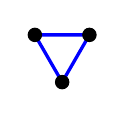
\begin{tikzpicture}[scale=0.5]
    \draw \foreach \x in {0,1,2}{(270+\x*360/3:0.8) coordinate(x\x)};
    \draw[edge_color2] (x0)--(x1)--(x2)--(x0);
    \draw (x0) node[unlabeled_vertex]{};
    \draw (x1) node[unlabeled_vertex]{};
    \draw (x2) node[unlabeled_vertex]{};
  \end{tikzpicture}}
}
\newcommand{\kthree}{\flagone}

\newcommand{\flagtwo}{ % this is the unlabeled edge
  \vc{
\begin{tikzpicture}[scale=0.5]
    \draw (225:0.8) coordinate(x0);
    \draw (45:0.8) coordinate(x1);
    \draw[edge_color2] (x0)--(x1);
    \draw (x0) node[unlabeled_vertex]{};
    \draw (x1) node[unlabeled_vertex]{};
  \end{tikzpicture}}
}
\newcommand{\edge}{\flagtwo}

\newcommand{\flagthree}{ % this represents the edges among non-neighbors of a vertex
  \vc{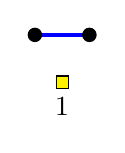
\begin{tikzpicture}[scale=0.5]
    \draw \foreach \x in {0,1,2}{(270+\x*360/3:0.8) coordinate(x\x)};
    \draw[edge_color2] (x1)--(x2);
    \draw (x0) node[labeled_vertex,label=below:$1$]{};
    \draw (x1) node[unlabeled_vertex]{};
    \draw (x2) node[unlabeled_vertex]{};
  \end{tikzpicture}}
}

\newcommand{\flagfour}{
  \vc{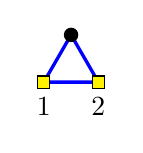
\begin{tikzpicture}[scale=0.5]
    \draw \foreach \x in {0,1,2}{(210+\x*360/3:0.8) coordinate(x\x)};
    \draw[edge_color2] (x0)--(x1)--(x2)--(x0);
    \draw (x0) node[labeled_vertex,label=below:$1$]{};
    \draw (x1) node[labeled_vertex,label=below:$2$]{};
    \draw (x2) node[unlabeled_vertex]{};
  \end{tikzpicture}}
}
\newcommand{\kthreeLabeledEdge}{\flagfour}

\newcommand{\flagfive}{ % this is the labeled edge
  \vc{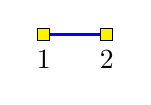
\begin{tikzpicture}[scale=0.5]
    \draw (180:0.8) coordinate(x0);
    \draw (360:0.8) coordinate(x1);
    \draw[edge_color2] (x0)--(x1);
    \draw (x0) node[labeled_vertex,label=below:$1$]{};
    \draw (x1) node[labeled_vertex,label=below:$2$]{};
  \end{tikzpicture}}
}
\newcommand{\labeledEdge}{\flagfive}

\newcommand{\flagsix}{ % this is the labeled non-edge
  \vc{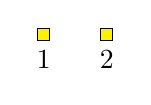
\begin{tikzpicture}[scale=0.5]
    \draw (180:0.8) coordinate(x0);
    \draw (360:0.8) coordinate(x1);
    \draw (x0) node[labeled_vertex,label=below:$1$]{};
    \draw (x1) node[labeled_vertex,label=below:$2$]{};
  \end{tikzpicture}}
}
\newcommand{\labeledNonEdge}{\flagsix}

\newcommand{\flagseven}{
  \vc{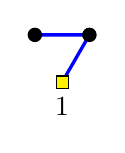
\begin{tikzpicture}[scale=0.5]
    \draw \foreach \x in {0,1,2}{(270+\x*360/3:0.8) coordinate(x\x)};
    \draw[edge_color2] (x0)--(x1)--(x2);
    \draw (x0) node[labeled_vertex,label=below:$1$]{};
    \draw (x1) node[unlabeled_vertex]{};
    \draw (x2) node[unlabeled_vertex]{};
  \end{tikzpicture}}
}

\newcommand{\flageight}{ % this is the labeled edge with an extra vertex joined to 1
  \vc{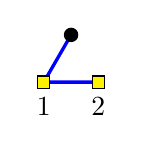
\begin{tikzpicture}[scale=0.5]
    \draw \foreach \x in {0,1,2}{(210+\x*360/3:0.8) coordinate(x\x)};
    \draw[edge_color2] (x2)--(x0)--(x1);
    \draw (x0) node[labeled_vertex,label=below:$1$]{};
    \draw (x1) node[labeled_vertex,label=below:$2$]{};
    \draw (x2) node[unlabeled_vertex]{};
  \end{tikzpicture}}
}

\newcommand{\flagnine}{ % this is the labeled edge with an extra vertex joined to 2
  \vc{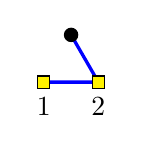
\begin{tikzpicture}[scale=0.5]
    \draw \foreach \x in {0,1,2}{(210+\x*360/3:0.8) coordinate(x\x)};
    \draw[edge_color2] (x0)--(x1)--(x2);
    \draw (x0) node[labeled_vertex,label=below:$1$]{};
    \draw (x1) node[labeled_vertex,label=below:$2$]{};
    \draw (x2) node[unlabeled_vertex]{};
  \end{tikzpicture}}
}

\newcommand{\flagten}{
  \vc{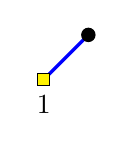
\begin{tikzpicture}[scale=0.5]
    \draw (225:0.8) coordinate(x0);
    \draw (45:0.8) coordinate(x1);
    \draw[edge_color2] (x0)--(x1);
    \draw (x0) node[labeled_vertex,label=below:$1$]{};
    \draw (x1) node[unlabeled_vertex]{};
  \end{tikzpicture}}
}
\newcommand{\edgeWithOneLabel}{\flagten}

\newcommand{\flageleven}{
  \vc{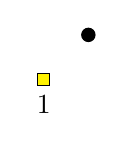
\begin{tikzpicture}[scale=0.5]
    \draw (225:0.8) coordinate(x0);
    \draw (45:0.8) coordinate(x1);
    \draw (x0) node[labeled_vertex,label=below:$1$]{};
    \draw (x1) node[unlabeled_vertex]{};
  \end{tikzpicture}}
}
\newcommand{\nonEdgeWithOneLabel}{\flageleven}

\newcommand{\flagtwelve}{
  \vc{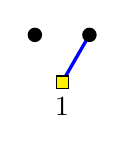
\begin{tikzpicture}[scale=0.5]
    \draw \foreach \x in {0,1,2}{(270+\x*360/3:0.8) coordinate(x\x)};
    \draw[edge_color2] (x0)--(x1);
    \draw (x0) node[labeled_vertex,label=below:$1$]{};
    \draw (x1) node[unlabeled_vertex]{};
    \draw (x2) node[unlabeled_vertex]{};
  \end{tikzpicture}}
}

A estrutura desse capítulo segue fortemente o que é apresentado em~\cite{marcel2016flag} e também inspirado nas lecture notes do Andrzej Grzesik.

\section{Preliminares}

Seja $k \geq 0$ um inteiro.
Um \emph{tipo} de \emph{tamanho} $k$ é um grafo $G$ com $V(G) = [k]$,
i.e. é um grafo com todos os seus vértices rotulados com os inteiros de $1$ a $k$.
O tipo vazio (grafo vazio) é denotado por $\emptyflag$.

Seja $\sigma$ um tipo de tamanho $k$ e $F$ um grafo com pelo menos $k$ vértices.
Um \emph{$\sigma$-flag} é um par $(F,\theta)$ em que $\theta \colon [k] \to V(F)$
é um homomorfismo de grafos injetor tal que $F[\theta([k])] \isom \sigma$.
Em outras palavras, $\sigma$-flag é um grafo \emph{parcialmente} rotulado, em que o subgrafo rotulado é uma cópia de $\sigma$.

Note que todo tipo $\sigma$ é um $(\sigma,\theta)$-flag para $\theta$ a função identidade em $[k]$.
Em geral, iremos omitir $\theta$ da definição de uma flag se a sua definição for clara do contexto.

Para definir isomorfismos entre $\sigma$-flags, fazemos exatamente como para grafos, com a condição adicional que os rótulo devem ser preservados pela bijeção.
Formalmente, dizemos que dois $\sigma$-flags $(G_1,\theta_1)$ e $(G_2,\theta_2)$ são \emph{isomórficos} se existe um isomorfismo $\theta \colon V(G_1) \to V(G_2)$ tal que $\theta(\theta_1(i))=\theta_2(i)$ para cada $i \in [|\sigma|]$.

\begin{example}

\begin{enumerate}
  \item Sejam \[\sigma_1=\labeledEdge \qquad \text{e} \qquad \sigma_2=\labeledNonEdge \]
  dois tipos (ambos com $k=2$ vértices).
  Então se $G=\kthreeLabeledEdge$ e $\theta$ é a identidade em $\{1,2\}$, temos que $(G,\theta)$ é um $\sigma_1$-flag mas não é um $\sigma_2$-flag.

  Usando a notação apresentada anteriormente, podemos simplesmente escrever que $G$ é um $\sigma_1$-flag.
  
  \item $\kthree$ é um $\emptyflag$-flag, uma vez que nenhum de seus vértices está rotulado.
  
  \item $\flagthree$ é um $\sigma_3$-flag, onde $\sigma_3$ é o (único) tipo com exatamente um vértice.
  $\flagseven$ é outro $\sigma_3$-flag.
  
  \item $\flageight$ e $\flagnine$ são dois $\labeledEdge$-flags, que são isomórficos como grafos mas não são isomórficos como flags.
\end{enumerate}

\end{example}

Finalmente, para cada tipo $\sigma$ e $n \geq |\sigma|$, definimos $\mathcal F_n^\sigma$ como o conjunto de todos os $\sigma$-flags de tamanho $n$.

\subsection{Densidade e limites}

Para continuar a definição de flag algebras, será importante definir densidades e suas propriedas.
Sejam $F$ e $G$ dois grafos (sem rótulos especiais nos vértices) e defina $c(F,G)$ como a quantidade de subgrafos \emph{induzidos} de $G$ que são isomorfos a $f$.
Então definimos a \emph{densidade de $F$ em $G$} como \[ p(F,G) \coloneqq \frac{c(F,G)}{\binom{|G|}{|F|}}. \]
De outra forma, $p(F;G) = \prob_U [G[U] \isom F]$ é a probabilidade que um subconjunto $U$ de $V(G)$ com tamanho exatamente $|F|$ induza um subgrafo isomorfo a $F$.

Por exemplo, temos $p(K_2;G) = \frac{e(G)}{\binom{n}{2}}$ e $p(K_3;G)$ é a probabilidade de uma tripla de vértices distintos de $G$ escolhida uniformemente ao acaso formar um triângulo.

De forma similar, para um tipo $\sigma$ dado, um $\sigma$-flag $(G,\theta)$ e um conjunto de $\sigma$-flags $F_1,F_2,\dots,F_t$, deifnimos a \emph{densidade de $F_1,F_2,\dots,F_t$ em $G$} como a probabilidade que conjuntos $U_1,U_2,\dots,U_t \subseteq V(G) \setminus \text{Im } \theta$ dois a dois disjuntos escolhidos uniformemente ao acaso satisfaçam $(G[U_i \cup \text{Im } \theta], \theta) \isom F_i$ para cada $i \in \{1,2,\dots,t\}$.
Denotamos essa densidade como $p(F_1,F_2,\dots,F_t;G)$.

\begin{example}
  Seja $\sigma$ o tipo de tamanho $1$.
  Sejam $F_1=\edgeWithOneLabel, F_2=\nonEdgeWithOneLabel, G=\flagseven$ três $\sigma$-flags.
  Então $p(F_1,F_2;G) = \frac12$.
\end{example}

Os dois seguintes lemas fornecem as relações para a ``regra da cadeia'' das densidades.

\begin{lemma}\label{lem:chain-rule-2}
  Sejam $F$ e $G$ dois $\sigma$-flags.
  Se $n$ é um inteiro positivo tal que $|F| \leq n \leq |G|$, então
  \[
    p(F;G) = \sum_{F' \in \mathcal F_n^\sigma} p(F;F')p(F';G).
  \]
\end{lemma}

\begin{lemma}\label{lem:chain-rule-many}
  Suponha que $F_1,F_2,\dots,F_t$ e $G$ são $\sigma$-flags.
  Se $n$ é um inteiro positivo tal que 
  \[
    \sum_{i=1}^t (|F_i|-|\sigma|) \leq n-|\sigma| \leq |G|-|\sigma|,
  \]
  então para todo $s \in [t]$ vale
  \[
    p(F_1,F_2,\dots,F_t;G) = \sum_{F \in \mathcal F_n^\sigma} p(F_1,F_2,\dots,F_s;F)p(F,F_{s+1},F_{s+2}\dots,F_t;G)
  \]
\end{lemma}

Agora, podemos definir a noção de funcionais limites e álgebras de flag.

\begin{definition}
  Uma sequência de grafos $(G_1,G_2,\dots)$ é chamada de \emph{crescente} se $(|G_1|,|G_2|,\dots)$ é estritamente crescente.
  Uma sequência crescente de grafos é chamada de \emph{convergente} se para todo grafo $F$ vale que a sequência
  \[ (p(F;G_1),p(F;G_2),\dots) \]
  é convergente.
\end{definition}

\begin{example}

\begin{enumerate}
  \item A sequência de grafos completos $(K_1,K_2,K_3,\dots)$ é convergente.
  \item A sequência de grafos bipartidos completos em que uma classe tem o tamanho da outra também é convergente: $(K_{1,2},K_{2,4},K_{3,6},\dots)$.
  \item A sequência de grafos de Andrásfai $(F_1,F_2,F_3,\dots)$ (que serão estudados no Capítulo~\ref{cap:grau-limitado}) é um exemplo menos trivial de sequência convergente.
\end{enumerate}

\end{example}

Sequências convergentes e crescentes de $\sigma$-flags são definidas de forma análoga para qualquer tipo $\sigma$.
Para cada sequência convergente de $\sigma$-flags $(A_1,A_2,\dots)$, podemos definir uma função $\phi$ que atribui a cada $\sigma$-flag $F$ o real $\phi(F) \coloneqq \lim_{k \to \infty} p(F;A_k)$.
A tais funções $\phi$ chamamos de \emph{limites funcionais}.

Na seção~\ref{sec:estrutura-algebrica}, iremos apresentar uma estrutura algébrica para flags the permitirão desenvolver propriedades gerais de limites funcionais.
Então, na seção~\ref{sec:aplicacoes}, mostraremos como traduzir os resultados obtidos para limites funcionais para a linguagem clássica de grafos e aplicá-las ao nosso problema.

\section{Estrutura algébrica}\label{sec:estrutura-algebrica}

Agora, vamos colocar uma estrutura algébrica para os flags.

Seja $\rfsigma$ o espaço vetorial gerado pelas combinações lineares de $\sigma$-flags com coeficientes (isto é, o espaço de somas formais de múltiplos reais de $\sigma$-flags).
Podemos estender linearmente qualquer limite funcional para $\rfsigma$.

Utilizando o Lema~\ref{lem:chain-rule-2}, obtém-se que para qualquer $\sigma$-flag $F$ e $n \geq |F|$ vale
\[ \phi(F) = \phi\left( \sum_{F' \in \mathcal F_n^\sigma} p(F;F') \right), \]
ou seja,
\[ F - \sum_{F' \in \mathcal F_n^\sigma} p(F;F') \]
is in the kernel of $\phi$ para todo funcional limite $\phi$.
We can then define the vector space $\asigma \coloneqq \rfsigma / \ker \phi$.
It is useful to note that $\phi(\sigma) = p(\sigma;F) = 1$ for every $\sigma$-flag $F$, so $\asigma$ has at least one nonzero element.

A principal vantagem de trabalhar com $\asigma$ é que é possível definir multiplicação entre seus elementos (transformando esse espaço vetorial em uma álgebra de fato).

\begin{definition}
  Sejam $F$ e $G$ $\sigma$-flags e seja $n \geq |F|+|G|-|\sigma|$.
  Definimos o produto de $F$ e $G$ como
  \[ F \cdot G = \left( \sum_{H \in \mathcal F_n^\sigma} p(F,G;H)H \right) \in \asigma. \]
\end{definition}

É possível provar que o produto acima está bem definido, é comutativo e associativo.

\begin{example}
  Sejam $F_1 = \edgeWithOneLabel$ e $F_2 = \nonEdgeWithOneLabel$. Então $F \cdot G = \frac12 \flagseven + \frac12 \flagtwelve$.
\end{example}

Agora, podemos enunciar o principal resultado das álgebras de flag.

\begin{theorem}[$\phi$ é homomorfismo de $\asigma$ para $\mathbb R)$]
  Se $f,g$ são dois elementos da álgebra $\asigma$ e $\phi$ é um funcional limite qualquer, então
  \[ \phi(f \cdot g) = \phi(f) \cdot \phi(g). \]
\end{theorem}

\section{Aplicações para a Conjectura \ref{conj:make-bipartite}}\label{sec:aplicacoes}

\begin{example}[Mantel]
  Se $\kthree = 0$, então $\edge \leq \frac12$.
\end{example}


\begin{theorem}
  Se $\kthree = 0$ e $\edge \geq \frac{2}{25}$, então
  $\left\llbracket
  \flagthree
  \right\rrbracket
  \leq \frac{2}{25}$.
\end{theorem}

\begin{corollary}
  Seja $G$ um grafo com $n$ vértices e pelo menos $\frac{n^2}{5}$ arestas.
  Então a Conjectura \ref{conj:make-bipartite} vale para $G$.
\end{corollary}

O ponto é que ter a linguagem de flag algebras facilita obter cotas a partir da ideia de ``cortes locais'' e daí pode automatizar o processo.

\begin{theorem}[Balogh-Clemen-Lidický]
  Seja $G$ um grafo livre de triângulos com $n$ vértices.
  Então, vale que
  \begin{enumerate}
    \item $D(G) \leq \frac{n^2}{23.5}$;
    \item $D(G) \leq \frac{n^2}{25}$ se $e(G) \geq 0.3197 \binom{n}{2}$;
    \item $D(G) \leq \frac{n^2}{25}$ se $e(G) \leq 0.2486 \binom{n}{2}$.
  \end{enumerate}
\end{theorem}
